\documentclass[12pt]{article}

% Specify document formatting.
\renewcommand{\baselinestretch}{1.5} 
\usepackage[top=2.5cm,bottom=2.5cm,inner=4cm,outer=2.5cm,twoside]{geometry}
\usepackage{fancyhdr} \usepackage{pdfpages} \usepackage[nottoc,notlof,notlot,numbib]{tocbibind}

% Change section title font size to 14.
\usepackage{sectsty}
\sectionfont{\fontsize{14}{15}\selectfont}

\usepackage{fontspec}
\setmainfont{Times New Roman}

\usepackage{amsmath} \usepackage{graphicx} \usepackage{microtype} \usepackage{float}
\usepackage[hidelinks]{hyperref} \usepackage{cleveref}
\usepackage{siunitx} \usepackage{gensymb}
\usepackage{tabularx} \usepackage{booktabs}
\usepackage[style=ieee]{biblatex} \addbibresource{zotero.bib}

\begin{document}
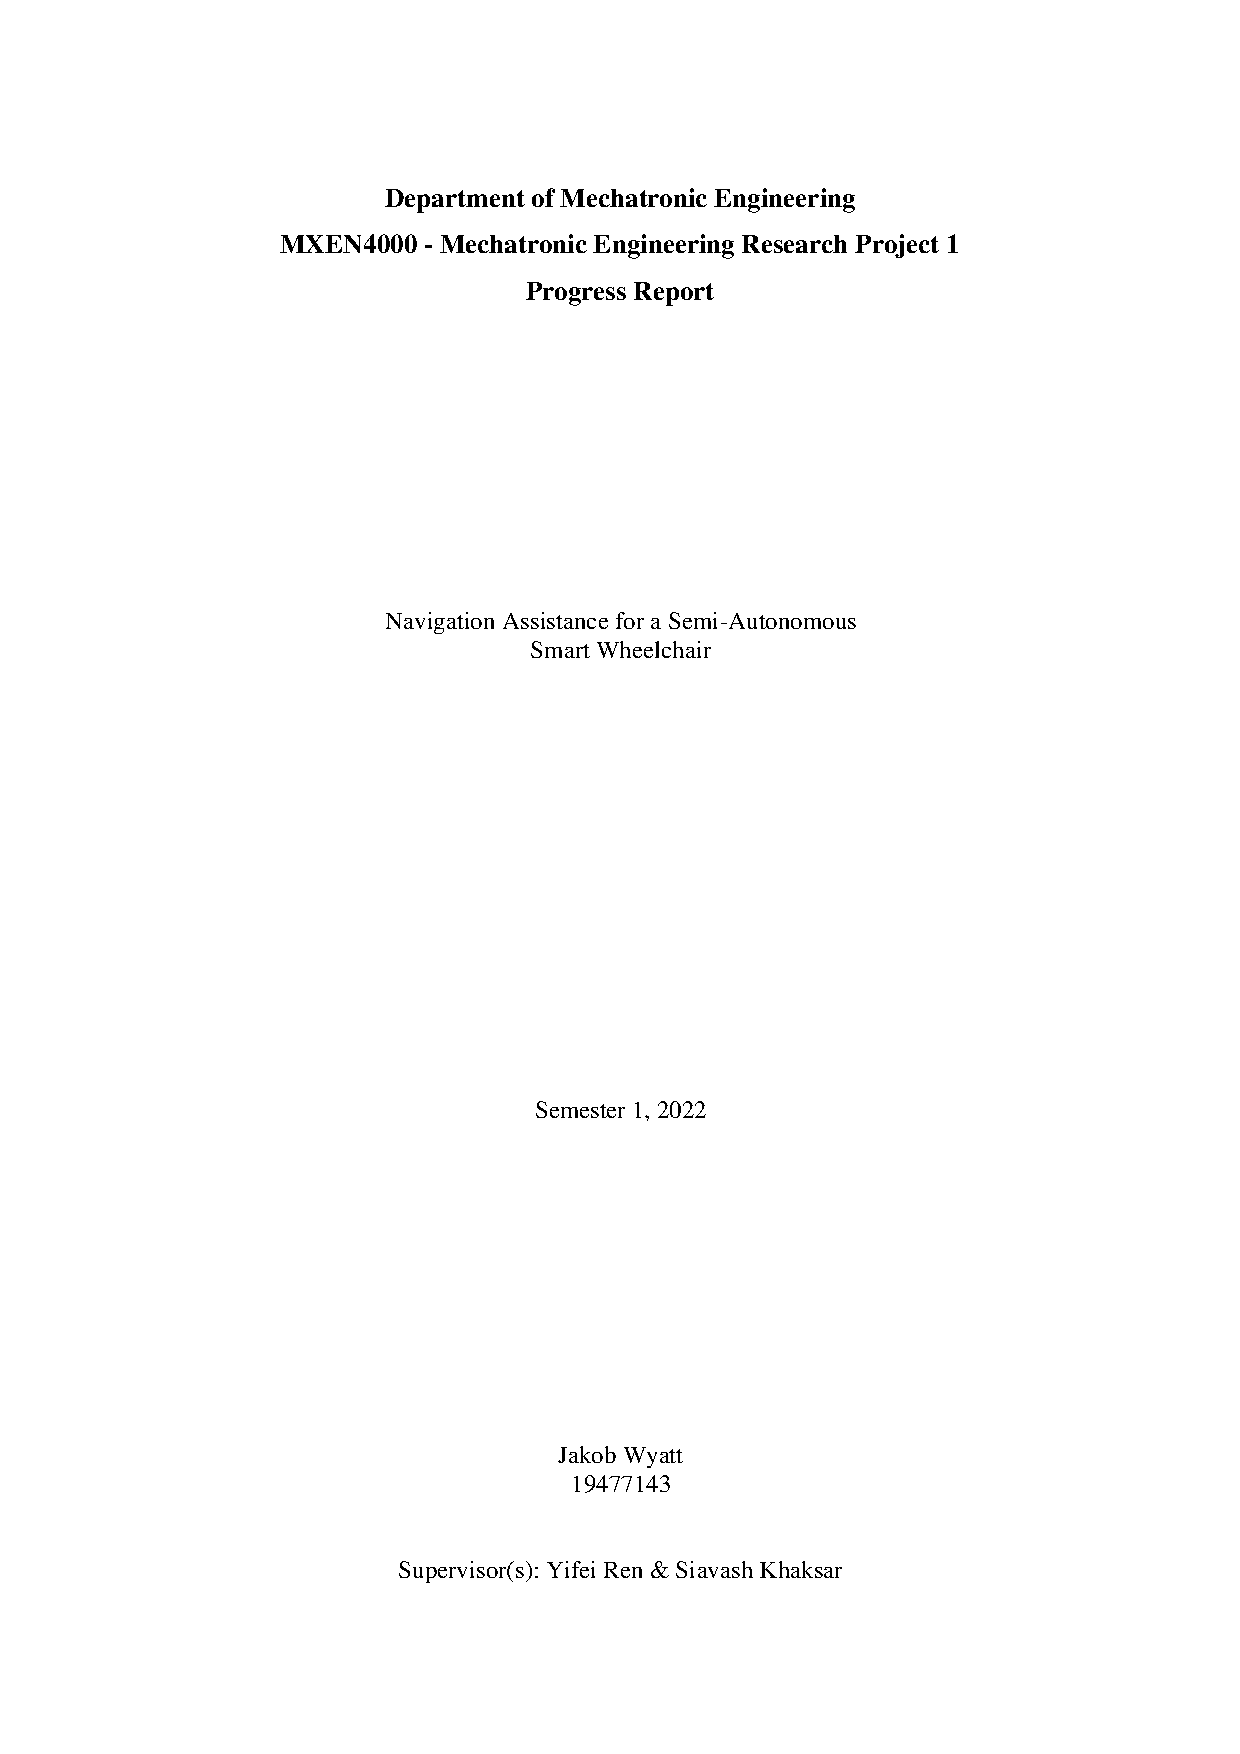
\includepdf{title.pdf}
\thispagestyle{empty}
\pagebreak

\pagenumbering{roman}
\section*{Abstract}
%\addcontentsline{toc}{section}{Abstract}
\pagebreak

\renewcommand{\contentsname}{Table of Contents}
\tableofcontents
\listoffigures
\listoftables
\pagebreak

\pagenumbering{arabic}
\section{Introduction}
Many people with motor disabilities rely on wheelchairs for movement, and
powered wheelchairs have enabled greater independance for people with disability.
Despite the huge benefit powered wheelchairs have granted,
the use of this technology can be inaccessible or unsafe for people
with amyotrophic lateral sclerosis (ALS) or vision impairment,
who may be unable to use a joystick or see their environment clearly.

\subsection{Aims}
The aim of this research is to develop a semi-autonomous smart wheelchair system.
This research is done in collaboration with Glide, a WA wheelchair manufacturer,
who have provided an existing powered wheelchair (CentroGlide) to use as a base
for this functionality. By developing assistive technology for the wheelchair,
the user is granted greater mobility, confidence, and independence.

\subsection{Problem Definition}
There are multiple engineering research project students who are part of this team,
working on elements such as controller design, navigation assistance, and object detection.
This work specifically focuses on pathway assistance, which identifies suitable
paths for the wheelchair to drive on. If a user unintentionally drives off their desired path,
this can lead to uneven terrain and possibly falling from the wheelchair.
By guiding the user along a path, these safety issues can be mitigated.

Emphasis is placed on the 'semi-autonomous' aspect of the wheelchair.
An important requirement of this project is that the user still
has control over their wheelchair, and can override any semi-autonomous functionality
if required. When false positives occur within the smart wheelchair system,
the users mobility should not be compromised.

Another requirement of the system is that any sensors mounted to the wheelchair
should not impede the users comfort or the wheelchairs manouverability.
Many wheelchair users have specific requirements for wheelchair seat adjustments,
to avoid pressure sores and discomfort. \Cref{fig:wheelchair_reclined} shows the
wheelchair configuration when fully reclined, demonstrating that some sensor mounting locations
are infeasible.

The smart wheelchair system should also be commercially viable - high-cost
components and sensors are infeasible. Internet connectivity should not be a requirement
for the system to operate either - the round trip time required to communicate with a server
would compromise the safety of a user. Because of this, all processing is performed locally
on the wheelchair.

\begin{figure}
    \centering
    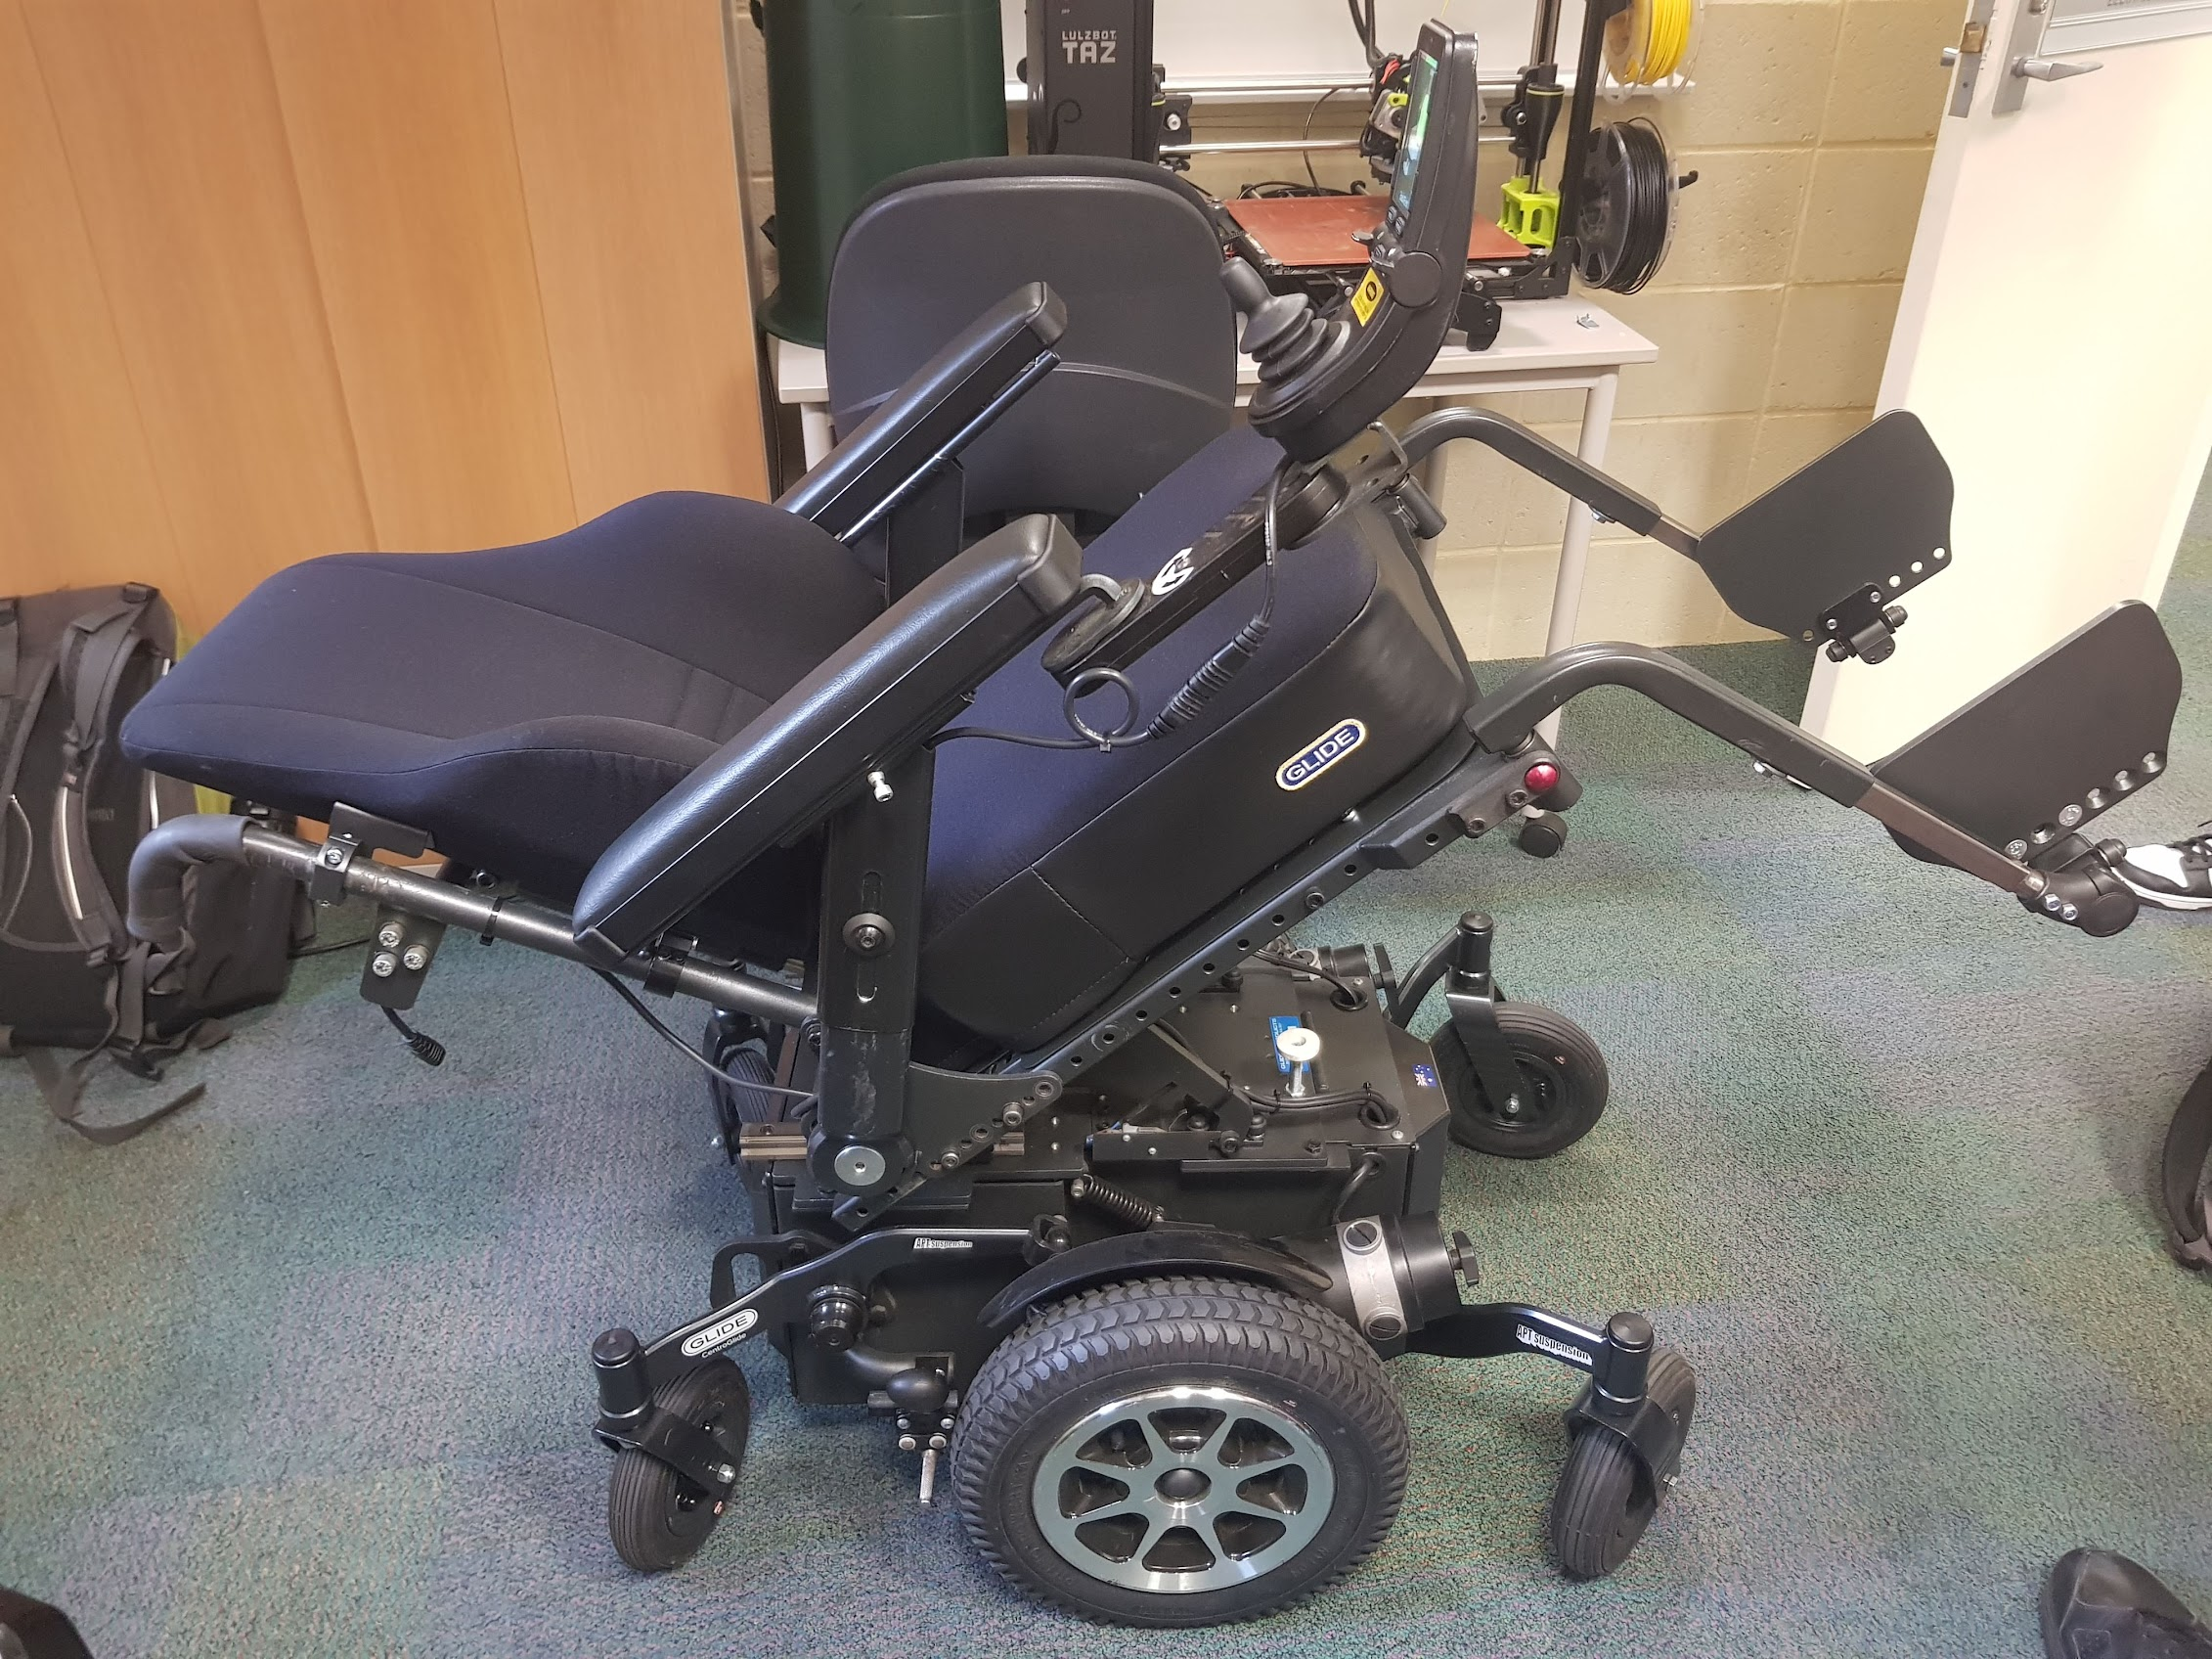
\includegraphics[width=0.8\linewidth]{images/wheelchair_reclined.jpeg}
    \caption{CentroGlide in Reclined Configuration}
    \label{fig:wheelchair_reclined}
\end{figure}
\pagebreak

\section{Literature Review}
%Smart wheelchairs are wheelchairs with additional sensors and computers,
%enabling greater usability and safety. This can come in the form of alternative input methods,
%such as eye-gaze tracking \cite{eidNovelEyeGazeControlledWheelchair2016} or using a brain-computer
%interface \cite{kaufmannBraincomputerInterfaceBased2014} to control the wheelchair. For people with vision impairment,
%haptic feedback \cite{kondoNavigationGuidanceControl2008}\cite{vanderpoortenPoweredWheelchairNavigation2012}
%has been used to improve awareness of the surrounding environment and make indoor navigation safer.

Initial research on semi-autonomous wheelchairs 

\subsection{Sensors and Hardware}
To percieve the environment, the wheelchair should be fitted with various sensors and
a compute element to process the sensors output. 

\Cref{table:sensor_options} shows some sensors that were considered for use in the smart wheelchair.
Selecting a sensor to use is not necessarily an either-or decision. Sensor fusion algorithms such as
the Extended Kalman Filter (EKF) or Unscented Kalman Filter (UKF) \cite{wanUnscentedKalmanFilter2000} allow
outputs from multiple sensors to be used together to improve their accuracy. Additionally, some sensors may
be used for different applications on the smart wheelchair.

\begin{table}
    \centering
    \begin{tabular}{c c c}
    \toprule
    Sensor & Advantages & Disadvantages \\
    \midrule
    Stereo Camera & High Resolution & \\
    MMWave Radar & & \\
    3D Lidar & & High Cost \\
    2D Lidar & & \\
    Ultrasonic Radar & & \\
    Inertial Measurement Unit (IMU) & & \\
    Servo Motor Encoder & & \\
    \bottomrule
    \end{tabular}
    \caption{Sensor Comparisons}
    \label{table:sensor_options}
\end{table}

\subsection{Scene Understanding}
Scene understanding is a broad field, and involves using computer vision methods
on visual or spatial data to gain better knowledge about the surrounding environment.
Convolutional Neural Networks (CNNs) are commonly used for this application, as they
are able to exploit the local nature of image features to reduce the number of required computations.

Image classification is a core sub-problem within this field, and involves identifying the
subject of an image (such as an animal or object).
AlexNet \cite{krizhevskyImageNetClassificationDeep2012} was one of the first deep CNNs
applied to this problem, performing well on the large ImageNet dataset \cite{jiadengImageNetLargescaleHierarchical2009}
with an error of only 15.3\%.
Neural network architectures have become deeper and more accurate over time, enabled by both
growth in computational power and dataset size.

For our application, we want to be able to . YOLO (You Only Look Once)

\subsection{Assistive Control}

% Inputs
% Semi-autonomy
% Full autonomy

% Indoor vs Outdoor assistance.
% Sensors
% Machine Learning
%\cite{tomariEnhancingWheelchairControl2014}
\pagebreak

\section{Methodology}
\subsection{Hardware}
The smart wheelchair should have the ability to sense, process, and manouver within the surrounding environment.
To do this requires some necessary hardware, including a sensor system, compute element, and motor controller.
Due to the 2021-2022 chip shortage, hardware selection was identified as a process that should occur relatively quickly.

The literature review provides a comparison between different sensor types and models. For outdoor navigation assistance,
a forward facing stereo camera was selected as the best option for this project - specifically, the Zed 2 Mini.
For the compute element, a Nvidia Jetson Xavier NX will be used, due to compatability with existing deep learning
frameworks and low power usage.

\subsection{Dataset Collection}
To train and evaluate machine learning models, a dataset was collected.
\pagebreak

\section{Current Work}
% 34 minute dataset
The first stages of smart wheelchair development involved:
\begin{enumerate}
    \item Identifying desired sensors and hardware for the wheelchair.
    \item Choosing an appropriate mounting point for these sensors.
    \item Researching the field of machine perception and computer vision (both applied to wheelchairs and more generally).
    \item Collecting an initial video dataset, enabling work to begin on labelling and algorithm evaluation.
\end{enumerate}

\subsection{Hardware}




After consideration of the available options, it was decided to use a stereo camera as the main
forward facing sensor, with 2D LIDAR used for the side and rear of the wheelchair.

The front of the joystick control unit was selected as the best mounting point for the
stereo camera, due to several reasons:
\begin{enumerate}
    \item Clear view of the environment in front of the wheelchair.
    \item Not obstructed by the user in any wheelchair configuration.
    \item When needed, the user can move the joystick control unit out of the way,
            which also moves the camera out of the way.
\end{enumerate}
However, there are some challenges faced when using this mounting point, which must be addressed.
\begin{enumerate}
    \item Shaky video footage due to low rigidity in joystick mount.
    \item Close to the front of the wheelchair, which reduces visibility of the sides of the wheelchair.
    \item Maximum camera width of \SI{150}{\milli\metre} before doorway manouverability is affected.
\end{enumerate}

To evaluate the effectiveness of this mounting point, a GoPro (Hero 4) was attached
using a temporary mount and a 34 minute driving dataset was collected around Curtin University.
% Images here
It was found that camera shakiness could be reduced by using a stiffer mounting solution,
however some shakiness would always remain due to the unstable mounting surface.
It was also found that alternative sensors, such as 2D LIDAR, would be required for features such as doorway
navigation and docking, due to the low field of view (FOV).

\pagebreak

\section{Future Work}
\pagebreak

\printbibliography[heading=bibnumbered]

\end{document}
